\subsection{Initializing the Directed Graph}
\begin{wrapfigure}{r}{0.35\linewidth} % Inline image example
	\begin{center}
		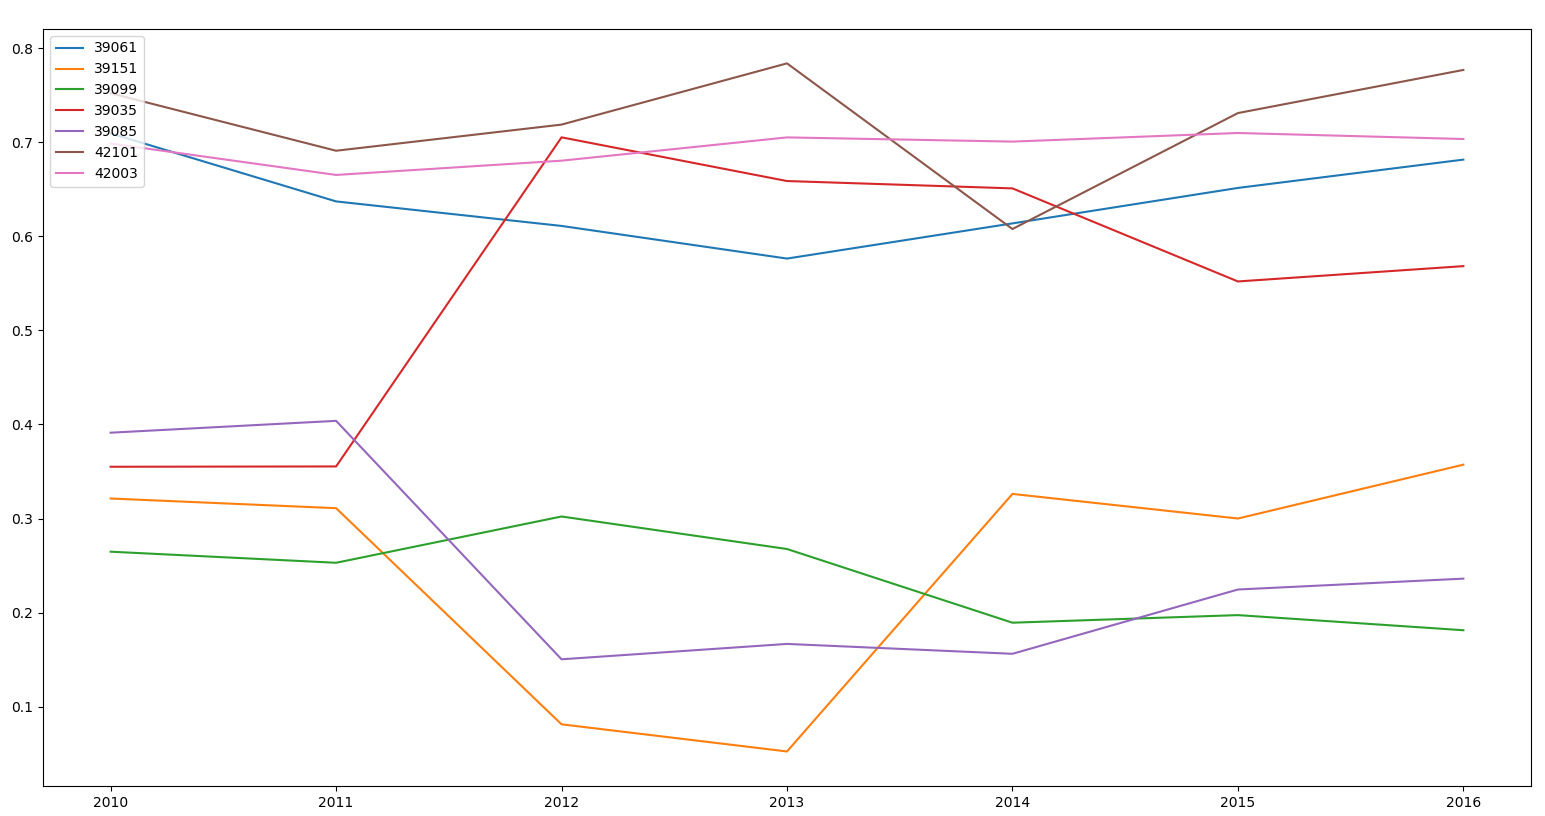
\includegraphics[width=\linewidth]{004}
	\end{center}
	\caption{$\lambda$ for the Seven Possible Origins}
\end{wrapfigure}

In the original Drug Spread Model, we temporarily overlooked the relationship between the parameter $\lambda$ and position $(x,y)$ in the formula. In this section, we modify our model so that $\lambda$ is strongly correlated with the socio-economic factors. 

Using the same algorithm introduced for locating the Possible Origin of specific opioid(see 4.3, Identify the Origin of Specific Opioid Use), we discovered the following seven Possible Origins for general Opioids.(see Table 9)

Since details concerning drug amount is inconsistent, and $\lambda=U/S$, we need to make the following assumptions to simplify our model in order to estimate the value of $\lambda$:

\begin{table}[H]
	\centering
	\begin{tabular}{|c|c|c||c|c|c|}
		\hline
		\rowcolor[HTML]{656565} 
		{\color[HTML]{FFFFFF} \textbf{STATE}} & {\color[HTML]{FFFFFF} \textbf{COUNTY}} & {\color[HTML]{FFFFFF} \textbf{F}} &{\color[HTML]{FFFFFF} \textbf{STATE}} & {\color[HTML]{FFFFFF} \textbf{COUNTY}} & {\color[HTML]{FFFFFF} \textbf{F}}\\ \hline
		KY & - & - &OH & Mahoning & 2115 \\ \hline
		VA & - & - &OH & Cuyahoga & 12190\\ \hline
		WV & - & - &OH& Lake &3003 \\ \hline
		OH & Hamilton & 11896 &PA & Philadelphia & 23431 \\ \hline
		OH & Stark & 2539 & PA & Allegheny & 8268 \\ \hline
	\end{tabular}
	\centering
	\caption{Possible Origins of Opioids in General}
\end{table}



\begin{enumerate}
	\item For Consumers, $\lambda \approx 1$. This indicates that Consumers have a limited ability to transport drugs out into neighboring counties, and can be omitted when conducting simplified calculations.
	
	\item Based on the above assumption, we can estimate $\lambda$ for Sources by
	\begin{equation}
	\lambda_{Source_i}=\frac{F_{Source_i}}{F_{Source_i}+\sum_{j\in N_i} F_{Consumer_j}}
	\end{equation} 
\end{enumerate}

\textit{
NOTE: In the following analysis, we abbreviate $\lambda_{Source_i}$ to $\lambda_i$, since we will mainly be considering the $\lambda$ value for Sources, and therefore no confusion shall occur. 
}

We computed $\lambda$ for the seven Possible Origins during 2010-2016(see Figure 2). In order to eliminate the effect that a steep variation might cause, we calculate $\overline{\lambda_i}$, which is the average $\lambda$ for each Possible Origin through 2010-2016:
\begin{table}[H]
	\centering
\begin{tabular}{|c|c|c|c|c|c|c|c|}
	\hline
	\rowcolor[HTML]{656565} 
	{\color[HTML]{FFFFFF} \textbf{SOURCE(FIPS Code)}} &{\color[HTML]{FFFFFF} \textbf{39061}} & {\color[HTML]{FFFFFF} \textbf{39151}} & {\color[HTML]{FFFFFF} \textbf{39099}}  & {\color[HTML]{FFFFFF} \textbf{39035}} & {\color[HTML]{FFFFFF} \textbf{39085}} & {\color[HTML]{FFFFFF} \textbf{42101}}  & {\color[HTML]{FFFFFF} \textbf{42003}}\\ \hline
	$\overline{\lambda}$ & 0.6401 & 0.2499 & 0.2365 & 0.5492 & 0.2470 & 0.7231 & 0.6948 \\ \hline
\end{tabular}
\centering
\caption{$\overline{\lambda_i}$ for the Seven Possible Origins}
\end{table}

As we can see in the table above, the $\overline{\lambda_i}$ obviously vary among the Possible Origins. We have
\begin{equation}
\overline{\lambda}=\frac{\sum_{t=1}^{7}\overline{\lambda_i}}{7}=0.4773
\end{equation}
therefore
\begin{equation}
\Delta \overline{\lambda_i} = \overline{\lambda_i} - \overline{\lambda}
\end{equation}
Our purpose here is to analyze which socio-econoic factors caused these differences.

\subsection{Prior Knowledge}
The ACS dataset provided more than five hundred possible factors, so feature extraction is obviously needed. 

A series of hypothesis have been developed to explain the socio-economic factors related to opioid use. Basing on statistics summarized by the American Addiction Center and other institutes\cite{10}\cite{11}, we obtain the following information:
\begin{itemize}
	\item \textbf{EDUCATION.} College graduates aged 26 or older battled drug addiction at lower rates than those who did not graduate from high school or those who didn’t finish college.
	\item \textbf{LONELINESS.} Those who live alone cope with drug addiction more than those who don't.
	\item \textbf{DISABILITY.} Those with a disability are more likely to be treated with opiods and thus more likely to become addicted.
	\item \textbf{GENDER/RACE.} Contradictory reports exist on the influence of gender and entity/race on obtaining drug addiction. 
	\item \textbf{POVERTY/UNEMPLOYMENT/FAMILY HISTORY.} Poverty, unemployment and family history are known risk factors of opioid misuse.
\end{itemize}


\begin{comment}
he above prior knowledge imply that education, loneliness, poverty, unemployment and family addiction history are the most influential factors. Contradicting reports regarding gender and entity factors allow us to assume that they play a minor part in opioid use.

Correspondingly, in the dataset, we choose \textit{\bfseries HC03\_VC85}(low educational background), \textit{\bfseries HC03\_VC14}(Nonfamily households - Householder living alone) and \textit{\bfseries HC01\_VC103}(DISABILITY STATUS OF THE CIVILIAN NONINSTITUTIONALIZED POPULATION - Total Civilian Noninstitutionalized Population). Let them be $Y_1$, $Y_2$ and $Y_3$ Further investigation showed that \textit{\bfseries HC01\_VC103} and all other disability-relevant factors were missing and therefore removed in the data cleansing proceidure. Therefore, we attempt to obtain $\lambda$ through linear regression by fitting
\begin{equation}
\lambda = \beta_1 Y_1 + \beta_2 Y_2
\end{equation}
\subsubsection{Linear Regression}
\end{comment}



%-------------------------------------

\subsection{Feature Extraction via LASSO}
We do not rely directly on prior knowledge to extract features related to $\lambda$, however. In order to derive useful information from the dataset, we use the LASSO method to observe how each factor contributes to $\lambda$. 

We consider the data from different years separately. Suppose that there are $N$ counties in the dataset, and each of these counties consists of $p$ \textbf{ \itshape covariates} (i.e. socio-economic factors). We map these covariates to the corresponding total drug use. In otherwords, the total drug use is denoted as the \textbf{ \itshape outcome}. Let $y_i$ be the outcome(i.e. $F_i(x,y)$ in this context) and $x_i = (x_1, x_2, \cdots, x_p)^T$ be the covariate vector for the $i_{th}$ case.

To guarantee the reliability of the data, we removed all margin errors and some other redundant features including ANCESTRY, LANGUAGE, YEAR OF ENTRY and PLACE OF BIRTH. More details were discussed in section 3, Addressing Missing Data.

The LASSO estimate is defined by\cite{7}
\begin{equation}
\hat{\beta}_{LASSO}=
\arg\min_{\beta} \sum_{i=1}^{N}(y_i - x_i^T\beta)^2 + \lambda'||\beta||_1
\end{equation}

subject to
\begin{equation}
 \sum_{j=1}^{p}|\beta_j|\leq t
\end{equation}

Here, $t$ determines the level of regularization. We fit the model using the coordinate descent algorithm. \cite{6}

We set the penalty factor $\lambda'$ to 1 to maximize the reduction in dimensions and extract the most valuble and relevant feature correlated with drug use. The LASSO result of five most influential features and their weights is shown in Table 11.

\begin{table}[H]
	\centering
	\begin{tabular}{|l|l|}
		\hline
		\rowcolor[HTML]{656565} 
		{\color[HTML]{FFFFFF} \textbf{FEATURE}} & {\color[HTML]{FFFFFF} \textbf{WEIGHT}} \\ \hline
		
		Estimate; SCHOOL ENROLLMENT - 	&2083.42 \\ 
		High school (grades 9-12) & \\ \hline
		
		Estimate; HOUSEHOLDS BY TYPE - 	& -1803.94 \\
		Family households (families) - Married-couple family & \\ \hline
		Estimate; HOUSEHOLDS BY TYPE -  &	-1580.07  \\ Households with one or more people under 18 years &\\ \hline
		Estimate; EDUCATIONAL ATTAINMENT - 	& 821.73 \\ 
		9th to 12th grade, no diploma & \\ \hline
		Estimate; HOUSEHOLDS BY TYPE - & 	800.73 \\
		Nonfamily households - Householder living alone & \\ \hline
		
	\end{tabular}
	\centering
	\caption{LASSO Results}
\end{table}

We can conclude from the above table that
\begin{enumerate}
	\item Lower education leads to drug use.
	\item A happy family(married, with children) has negative correlation with drug usage. On the contrary, nonfamily households where householders live alone has a positive correlation.
\end{enumerate}

\subsection{Comparison Between Prior Knowledge and LASSO Results}
Based on reliable prior knowledge, those with a disability are more likely to use/misuse opioids. Even though there are features concerning disability in our dataset, vast amount of information is missing(we dealt with this problem in Data Processing, Section 3). 

As for possible influential factors like poverty, unemployment and family history, they are inanalyzable since no such data appeared in our dataset.

Contradicting hypothesis exist concerning the influence of gender and race on drug usage, so we neglect these factors in our model.

To sum up, we emphasize on \textbf{EDUCATION} and \textbf{LONELINESS}. 
\subsubsection{Education}
We combine feature \textit{Percent; EDUCATIONAL ATTAINMENT - Less than 9th grade} and \textit{Percent; EDUCATIONAL ATTAINMENT - 9th to 12th grade, no diploma} into one single feature named \textit{Percent; EDUCATIONAL ATTAINMENT - Less than 12th grade, no diploma}.
\subsubsection{Loneliness}
We could consider features which are positively or negatively correlated with drug use at the same time, but this might affect the independence between features. Thus we chose the positively correlated feature \textit{Percent; HOUSEHOLDS BY TYPE - Nonfamily households - Householdgger living alone} to address loneliness.

\subsection{Linear Regression}
Next, we examine how education and loneliness contribute to $\lambda$ through linear regression.


\begin{wrapfigure}{r}{0.35\linewidth} % Inline image example
	\begin{center}
		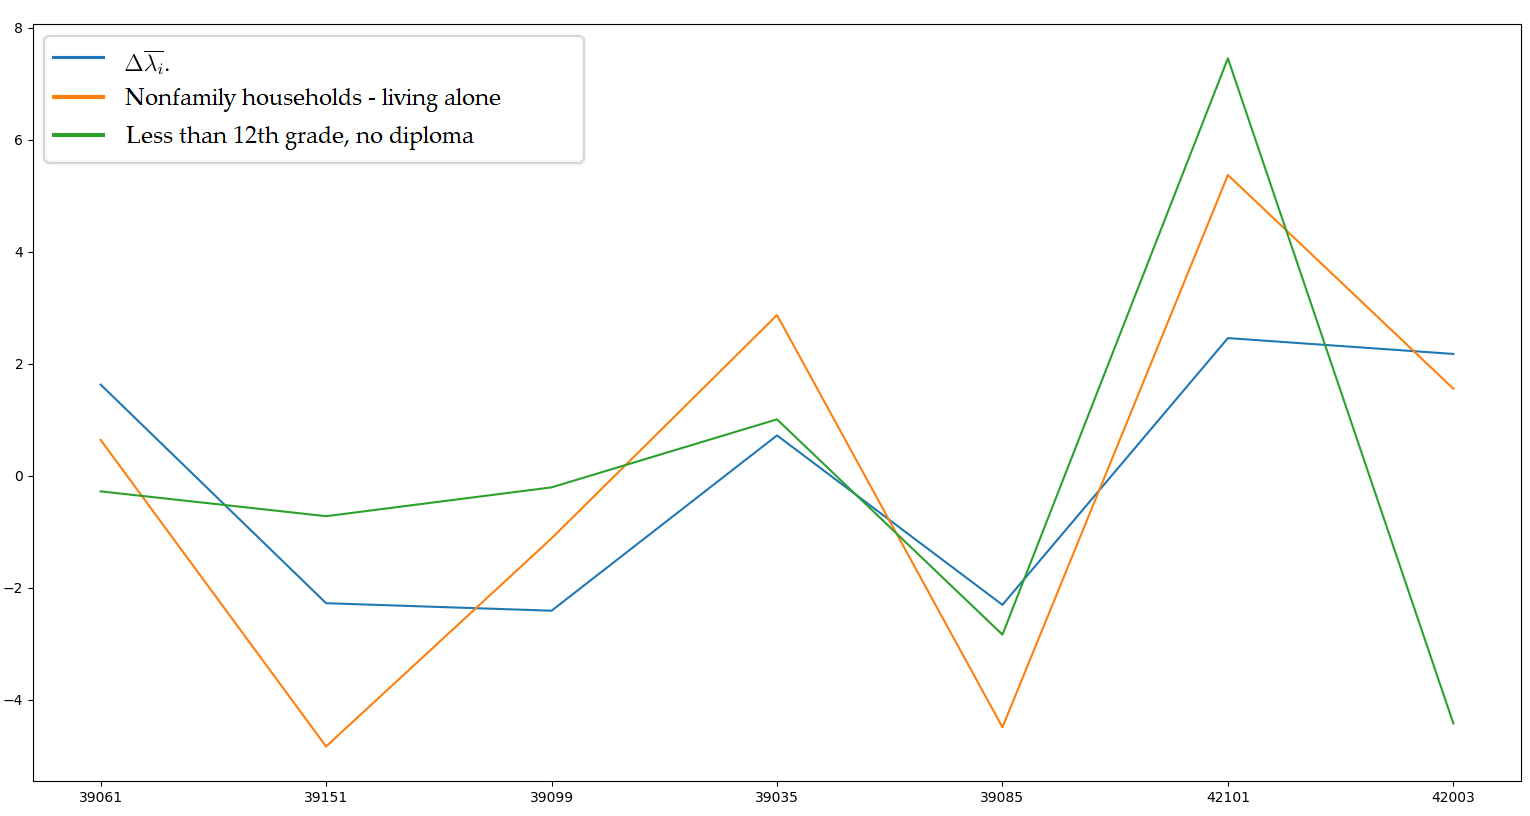
\includegraphics[width=\linewidth]{005}
	\end{center}
	\caption{the relationship between $\Delta \overline{\lambda_i}$, $\Delta \overline{y_{1i}}$ and  $\Delta \overline{y_{2i}}$}
\end{wrapfigure}


When appling the LASSO method, we choose $F$ as the training target. $F$ is a digital value, so all features correlated with it are estimated digital values. However, when we take into acoount of the fact that $\lambda$ is defined by proportion, it seems more adequate for us to choose percentages which makes sense both in magnitude and actual meaning.


The target of linear regression is $\Delta \overline{\lambda_i}$. We conduct similar operations on each feature, and denote them as $\Delta \overline{y_{1i}}$ and  $\Delta \overline{y_{2i}}$. Before finally computing the linear regression result, we visualize the relationship between $\Delta \overline{\lambda_i}$, $\Delta \overline{y_{1i}}$ and  $\Delta \overline{y_{2i}}$.(Figure 3).

From the consistency of the three attributes shown in the figure, it is obvious that $\Delta \overline{\lambda_i}$, $\Delta \overline{y_{1i}}$ and  $\Delta \overline{y_{2i}}$ are indeed positively correlated. Thus, our linear regression model can be described as
\begin{equation}
\Delta \overline{\lambda_i} = k_1 \Delta \overline{y_{1i}} + k_2 \Delta \overline{y_{2i}} + k3
\end{equation}

The solution to equation (20) is
\begin{equation}
\left\{
\begin{array}{l}
k_1 = a \\
k_2 = b \\
k_3 = c \\
\end{array}
\right.
\end{equation}

Equation (20) describes how socio-economic factors affect our Drug Spread Model from a quantitative point of view. When the actual value of data F is not available, we would still be able to estimate the Sources' $\lambda$ through socio-economic factors.

